% Totoro sitting in the snow
% By Noa Hoffmann and Pascal Günthner, 21.12.2020
\documentclass[tikz,11pt]{{standalone}}
\usepackage{calligra}
\usepackage[T1]{fontenc}
\usetikzlibrary{positioning, chains, calc, fit, arrows.meta, shapes}

\begin{document}    
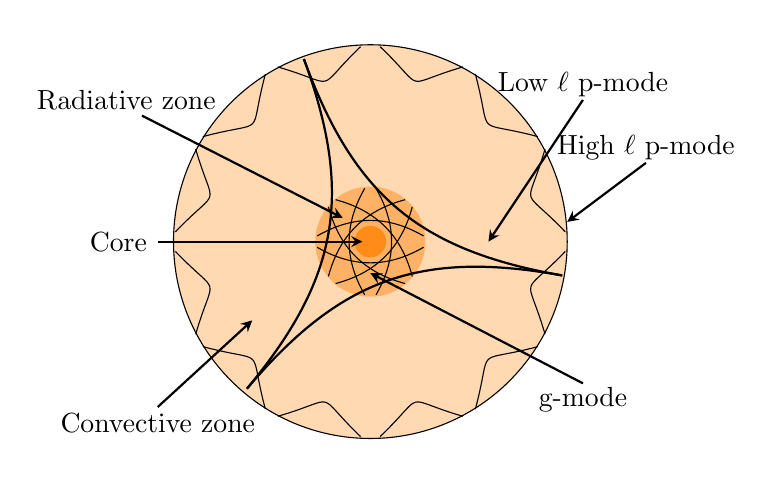
\begin{tikzpicture}
    \coordinate (O) at (0,0);
    \draw[fill=orange!30] (O) circle (2.5);
    \draw[fill=orange!60, draw=none] (O) circle (0.7);
    \draw[fill=orange!90, draw=none] (O) circle (0.2);
    \draw[stealth-, thick](-0.1, 0) -- (-2.7, 0);
    \draw[stealth-, thick](-0.35, 0.3) -- (-2.9, 1.6);
    \draw[stealth-, thick](-1.5, -1.) -- (-2.7, -2.1);
    \draw(-3.2, 0) node {Core};
    \draw(-3.1, 1.8) node {Radiative zone};
    \draw(-2.7, -2.3) node {Convective zone};   
    \draw[stealth-, thick](1.5, -0.0) -- (2.7, 1.8);
    \draw(2.7, 2.) node {Low $\ell$ p-mode};
    \draw[stealth-, thick](-0.0, -0.4) -- (2.7, -1.8);
    \draw(2.7, -2.) node {g-mode};
    \draw[stealth-, thick](2.5, 0.25) -- (3.5, 1.);
    \draw(3.5, 1.2) node {High $\ell$ p-mode};
     \foreach \i in {1,2,3} {
     \node[] (p\i) at ($(O)+(360*\i/3-10:2.6)$)  {};
     }
     \foreach \i/\j in {1/2,2/3,3/1}{
     \draw [black, bend left, looseness=1.1, thick] (p\i) edge (p\j); 
     }
     \foreach \i in {1,2,3,4,5,6,7,8} {
     \node (p\i) at ($(O)+(360*\i/8:0.8)$) {};
     }
     \foreach \i/\j in {1/5,2/6,3/7,4/8,5/1,6/2,7/3,8/4}{
     \draw [black, bend right, looseness=1.] (p\i) to (p\j); 
     }
     \foreach \i in {1,2,3,4,5,6,7,8,9,10,11,12} {
     \node[] (p\i) at ($(O)+(360*\i/12:2.6)$)  {};
     }
     \foreach \i/\j in {1/2,2/3,3/4,4/5,5/6,6/7,7/8,8/9,9/10,10/11,11/12,12/1}{
     \draw [black, bend left, looseness=2.] (p\i) edge (p\j); 
     }
    % \draw[black] (0,0.7) to[curve through={(-0.45,0.25)..(-0.1,0) .. (0.1,0) .. (0.45,0.35)}] (0,0.7);
\end{tikzpicture}
\end{document}
